%% LyX 2.2.0dev created this file.  For more info, see http://www.lyx.org/.
%% Do not edit unless you really know what you are doing.
\documentclass{IEEEtran}
\usepackage[latin9]{inputenc}
\usepackage[letterpaper]{geometry}
\geometry{verbose,tmargin=1in,bmargin=1in,lmargin=1in,rmargin=1in}
\setlength{\parskip}{\smallskipamount}
\setlength{\parindent}{0pt}
\usepackage{color}
\usepackage{float}
\usepackage{textcomp}
\usepackage{graphicx}
\usepackage[authoryear]{natbib}
\usepackage[unicode=true,pdfusetitle,
 bookmarks=true,bookmarksnumbered=false,bookmarksopen=false,
 breaklinks=true,pdfborder={0 0 0},backref=false,colorlinks=true]
 {hyperref}
\hypersetup{
 linkcolor=blue,urlcolor=blue,citecolor=blue}
 \usepackage{gensymb}
 \usepackage{comment}

\makeatletter
%%%%%%%%%%%%%%%%%%%%%%%%%%%%%% User specified LaTeX commands.
\usepackage{color}%% maxwidth is the original width if it is less than linewidth
%% otherwise use linewidth (to make sure the graphics do not exceed the margin)

\def\maxwidth{ %
  \ifdim\Gin@nat@width>\linewidth
    \linewidth
  \else
    \Gin@nat@width
  \fi
}


\definecolor{fgcolor}{rgb}{0.2, 0.2, 0.2}
\newcommand{\hlnumber}[1]{\textcolor[rgb]{0,0,0}{#1}}%
\newcommand{\hlfunctioncall}[1]{\textcolor[rgb]{0.501960784313725,0,0.329411764705882}{\textbf{#1}}}%
\newcommand{\hlstring}[1]{\textcolor[rgb]{0.6,0.6,1}{#1}}%
\newcommand{\hlkeyword}[1]{\textcolor[rgb]{0,0,0}{\textbf{#1}}}%
\newcommand{\hlargument}[1]{\textcolor[rgb]{0.690196078431373,0.250980392156863,0.0196078431372549}{#1}}%
\newcommand{\hlcomment}[1]{\textcolor[rgb]{0.180392156862745,0.6,0.341176470588235}{#1}}%
\newcommand{\hlroxygencomment}[1]{\textcolor[rgb]{0.43921568627451,0.47843137254902,0.701960784313725}{#1}}%
\newcommand{\hlformalargs}[1]{\textcolor[rgb]{0.690196078431373,0.250980392156863,0.0196078431372549}{#1}}%
\newcommand{\hleqformalargs}[1]{\textcolor[rgb]{0.690196078431373,0.250980392156863,0.0196078431372549}{#1}}%
\newcommand{\hlassignement}[1]{\textcolor[rgb]{0,0,0}{\textbf{#1}}}%
\newcommand{\hlpackage}[1]{\textcolor[rgb]{0.588235294117647,0.709803921568627,0.145098039215686}{#1}}%
\newcommand{\hlslot}[1]{\textit{#1}}%
\newcommand{\hlsymbol}[1]{\textcolor[rgb]{0,0,0}{#1}}%
\newcommand{\hlprompt}[1]{\textcolor[rgb]{0.2,0.2,0.2}{#1}}%

\usepackage{framed}
\newenvironment{kframe}{%
 \def\at@end@of@kframe{}%
 \ifinner\ifhmode%
  \def\at@end@of@kframe{\end{minipage}}%
  \begin{minipage}{\columnwidth}%
 \fi\fi%
 \def\FrameCommand##1{\hskip\@totalleftmargin \hskip-\fboxsep
 \colorbox{shadecolor}{##1}\hskip-\fboxsep
     % There is no \\@totalrightmargin, so:
     \hskip-\linewidth \hskip-\@totalleftmargin \hskip\columnwidth}%
 \MakeFramed {\advance\hsize-\width
   \@totalleftmargin\z@ \linewidth\hsize
   \@setminipage}}{\par\unskip\endMakeFramed%
 \at@end@of@kframe}



\definecolor{messagecolor}{rgb}{0, 0, 0}
\definecolor{warningcolor}{rgb}{1, 0, 1}
\definecolor{errorcolor}{rgb}{1, 0, 0}
\newenvironment{knitrout}{}{} % an empty environment to be redefined in TeX

\usepackage{alltt}\usepackage{booktabs}\usepackage{fullpage}


% Create a new command, \blfootnote which creates a footnote without a number
\newcommand{\blfootnote}[1]{%
  \begingroup
  \renewcommand\thefootnote{}\footnote{#1}%
  \addtocounter{footnote}{-1}%
  \endgroup
}
\IfFileExists{upquote.sty}{\usepackage{upquote}}{}

\makeatother

\begin{document}

\title{{\small{}Guam New Invasive Species Alert No. 2016-01}{\Huge{}}\\
{\Huge{}Greater Banded Hornet}\textit{\huge{}}\\
\textit{\huge{}Vespa tropica}{\huge{}}\\
{\huge{}(Hymenoptera: Vespidae) }}

\author{Christopher A. Rosario, Lee Roy Sablan, Ross H. Miller, and Aubrey Moore\\
 University of Guam, College of Natural and Applied Sciences\\
 July 13, 2016\\Updated August 10, 2016}

\maketitle

\begin{figure}[H]
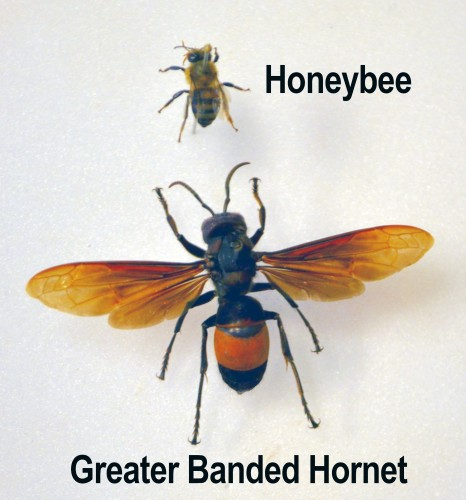
\includegraphics[width=\columnwidth]{Hornet_bee500.jpg}
\protect\caption{\label{fig:vespa-tropica}The first greater banded hornet collected on Guam with a honeybee for size comparison. Photo by Olympia Terral. }
\end{figure}


On July 12, 2016, University of Guam research assistant Christopher Rosario discovered a colony of large wasps nesting in a hollow avocado tree in Dededo, Guam (13.50533 \degree N, 144.80134 \degree E). The wasps were aggressive, resulting in only single specimen being collected. This observation was posted on the iNaturalist web site (\url{http://www.inaturalist.org/observations/3663868}).

On July 20, 2016, Arnold Perez of the Leo Palace Resort delivered 5 specimens of \textit{Vespa tropica} to Dr. Aubrey Moore at the University of Guam. Perez discovered a nest near a swiiming pool (\url{http://www.inaturalist.org/observations/3710757}). Specimens were placed in the University of Guam Insect Collection.

On August 8, 2016, Joey Lopez submitted an image of \textit{V. tropica} collected at the Sheraton Hotel on Guam from (\url{http://www.inaturalist.org/observations/3846302}).


\section*{Description}

UOG entomologists identified the wasp as \textit{Vespa tropica} based on publicly available images and keys \citep{archer1991taxonomy}. This is a medium-sized to large species. Queens reach 30mm or more, males average 26mm and workers average 24 to 26mm. 

This species is known to attack the nests of Polistines (paper wasps) in order to obtain the larvae to feed their own larvae. It is said to be almost exclusive in choice of prey. However, they sometimes catch honeybees

The nest of \textit{Vespa tropica} is usually underground or in a tree hollow or similar enclosed space. Due to the location, the nest is seldom seen. If excavated, the nest usually appears rhomboid or bowl-shaped, with an open bottom (as opposed to the completely sealed nests of most aerial hornets). The nest envelope is laminar (comprising of distinct, broad individual layers) and very brittle.

\section*{Distribution}

\textit{Vespa tropica} is found in China, Japan, Malaysia, Hong Kong, Singapore, India, and the Philippines \citep{GBIF}.

%\section*{Acknowledgments}

%Acknowledgments to appear here.

\newpage{}
\bibliographystyle{plainnat}
\nocite{*}
\bibliography{VespaTropica}

\end{document}